\documentclass{../download/tPRS2e}

    \usepackage[english]{babel}
    \usepackage{tikz}
    \usetikzlibrary{patterns}
    \usepackage{graphicx}
    \graphicspath{{media/}}
    
\begin{document}

\title{On the Problem of Tool Air Move Minimization for Sheet Cutting CNC Machine}

\author{
\name{
Petunin A.A.\textsuperscript{a},
Polishuk E.G.\textsuperscript{a},
Ukolov S.S.\textsuperscript{a}$^{\ast}$\thanks{$^\ast$Corresponding author. Email: s.s.ukolov@urfu.ru}
}
\affil{
\textsuperscript{a}Ural Federal University, Yekaterinburg, Russia;
}}

\maketitle

\begin{abstract}
The problem of finding pierce points to get
minimal tool air move path length is considered
in case of standard cutting technique
(closed contours cutting).
Discrete approximation is discussed,
then a new algorithm is described,
which perform no discretization,
i.e. any point on a contour can be 
used for piercing operation.
\end{abstract}

\begin{keywords}
    contour;
    pierce point;
    minimal tool path;
    sheet cutting CNC machine;
\end{keywords}

\section{Introduction}

During development of control programs for
CNC sheet cutting machines,
the problem of minimizing tool idle path
often appears.
One should select the order
of part contours to cut
and positions of pierce point on them,
so as total length of tool trajectory be minimal,
which implies,
that length of broken line connecting all
pierce points in the order of contour cutting
also be minimal.
In addition, a technological requierment should be met,
that if some contour lays inside another one,
the former must be processed before the latter.

\section{Precedence constraint handling}

Note, that we can consider
only contours containing no inner sub-contours.
Having got a solution for these contours,
one can easily add vertices
(pierce points) for the other contours,
preserving total length of the broken line.

\begin{enumerate}
    \item{}
To see this, let us denote by
$L_f$ the broken line length for original task
(for all contours considered)
and by 
$L_0$ that length for task with reduced set of contours.
Next we denote with $M$ and $N$
two vertices of the broken line for original task
($L_f$),
so as they belongs to remaining contours.
We can remove all intermediate links and connect 
$M$ to $N$ with line segment,
getting a new broken line with less or equal length.
So, $L_f \ge L_0$.
    \item{}
Let us consider broken line
having no vertex on some contour $C$.
One can find the \textbf{last} segment
of the broken line
that inersects $C$.
At least one such segment is known to exist,
because there is another contour inside $C$,
which in turn contains one vertex of the broken line.
The point of intersection $C \cap L_0$ can be inserted
into the broken line as new vertex,
giving a new broken line with the same length $L_0$
containg a vertex laying on the $C$.
Repeating this operation for all outer contours,
we get broken line $L_f$ with the same length
which conforms to above
technological constraint.
\end{enumerate}

Finally, $L_f = L_0$ and we can solve the problem,
considering only non-outer contours.

\section{Pierce point positioning}

When the order of contours is fixed,
the problem reduces to the following:

There are $n$ closed contours
$C_1, C_2, \dots C_n$ on Euclidean plane
$\mathbb R^2$.
Each contour consists of finite number of links,
i.e. linear segments and arcs.
Among all broken lines $\{M_1, M_2, \dots M_n\}$
(where vertice $M_i$ belongs to a circuit $C_i$,
$i = 1, 2, \dots n$),
we look for the shortest one.

This inherently continuous problem can be approximated
by the discrete one [1]
reffered to as \textit{General Travelling Salesman Problem}
(GTSP).
We choose fixed $\varepsilon$ and break all the contours
into segments of length $\varepsilon$ (or less),
then our minimization problem is solved for the 
broken lines, whose vertices are selected from the
breaking points. Note, that
$$
L \le L_\varepsilon \le L + \frac{\varepsilon}2 n
$$
where $L$ is the length of broken line for original
(continuous) problew,
while $L_\varepsilon$ is that for discrete one.
To be sure, that
$| L - L_\varepsilon | < \delta $
for some fixed $\delta$,
one should select $\varepsilon = 2 \delta /n$.
For big $n$ this $\varepsilon$ is small hence
the number of possible vertices is large.
Such a problem can be solved using dynamic programming
with time requirements of
$O(m_1 \cdot m_2^2 \cdot \dots m_{n-1}^2 \cdot m_n)$,
where $m_i$ is a number of discretization points on the
contour $C_i$.
Thus, low $\delta$ yields large $n$ and long
calculation time.

Instead we can directly solve original
(continuous) problem as discussed below.

An initial broken line is somehow constructed.
We will gradually improve it.
One step of iteraton is:

For $ \forall i = 1, 2, \dots n$ we try to move vertex $M_i$
along contour $C_i$ in order to minimize total length
of broken line. All other vertices are fixed.
This problem can be thus stated:
find the point on the line segment (or arc)
that minimizes sum of distances from it to
two other fixed points.

All possible dispositions of points around the contour
are simply enumerated and analyzed.
We highlight the only one case,
when both fixed points are situated on the one side
of the straight line containing segment of a contour.
Here the Fermat principle applies
(\textit{the angle of incidence is equal to the reflex angle}).

Note, that like any descent algorithm of optimization,
this cannot guarantee
the global minimum can be obtained,
but ensures that found broken line is a local minimum.
We can run relaxation from several different initial broken lines,
checking all of them give the same solution.

\section{Order of contours to process}

For approximate solution of main problem
that includes finding order of contours to cut,
the following process is proposed:

An initial ordering is constructed by selecting 
nearest contour to the current one as next to it.
Pierce points for all contours 
(vertices of broken line) are positioned arbitrarily.
Then, relaxation of this initial broken line 
is performed to find solution with minimal length.
This is done by considering several permutations
of initial ordering and optimal pierce point positions
are calculated as stated above.
When new broken line is found
that has shorter total length,
it replaces the initial one and process is restarted.

\begin{enumerate}
    \item{All permutation of two or three contours are processed}
    \item{Shifts of blocks (several sequential contours) in several steps back and / or forward are applied}
    \item{Ordering inside blocks is reversed}
\end{enumerate}

During relaxation to minimal path length,
additional heuristic can be applied:
if in attempt to rearrange some contours,
the length of a polyline constructed
only for these contours is longer than the current one,
then no permutations containing this are considered.

\section{Results}

During numerical experiments,
performance of algorithm described
was compared to that reffered in [1]
(heuristics for GTSP solving
using discretized pierce point positions).
In general, our approach gives an improvement of 10\% to 20\%.

See result of [1] at Fig. \ref{dynprog}
\textit{cf} our result at Fig. \ref{heuristics}.

For some other nestings comparison is summarised in Table \ref{exact-3}.
In this case a low number or contours is used
(below 30),
so exact GTSP solution can be found.
We can see,
that solution found by our algorithms
is both local and global optimum.

Resulting tool path is slightly shorter,
because we can route cutting head along straight lines
whereas GTSP's tool path is always polygonal
due to preliminary discretization involved.

\begin{figure}[]
    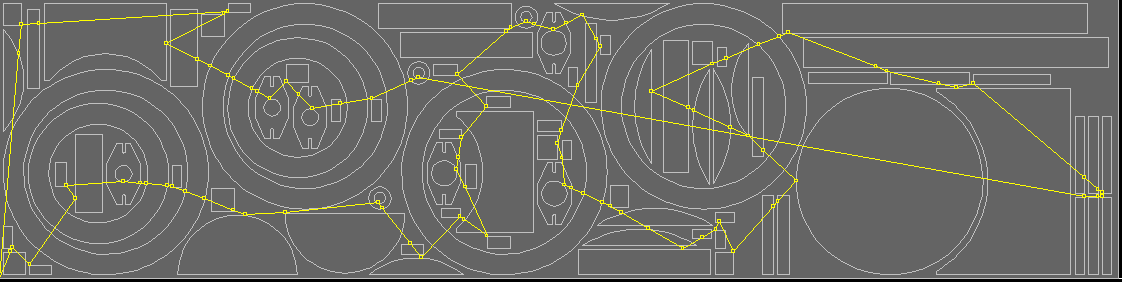
\includegraphics[width=0.95\textwidth]{mini-bad.png}
    \caption{GTSP solution. Total length of path is 19649 mm}
    \label{dynprog}
\end{figure}

\begin{figure}[]
    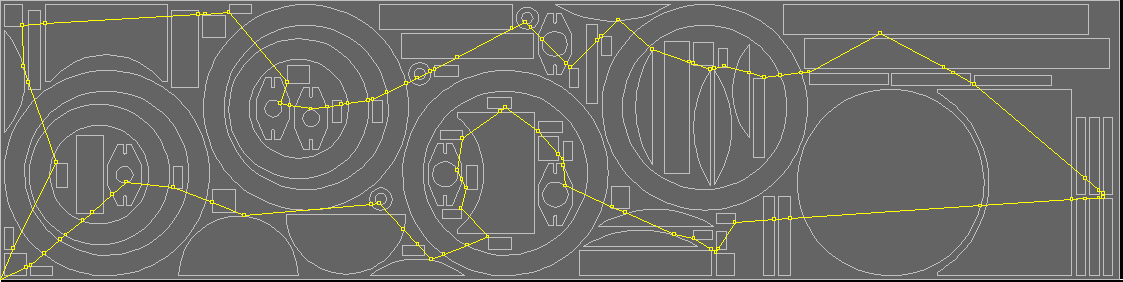
\includegraphics[width=0.95\textwidth]{mini-good.png}
    \caption{Our solution. Total length of path is 15836 mm}
    \label{heuristics}
\end{figure}

\begin{table}[h]
    \begin{center}    
    \begin{tabular}{l|*{3}{r}}
        Job & \#229 & \#464 & \#3211 \\
        \hline
        \# of parts & 11 & 14 & 17\\
        \# of contours & 12 & 21 & 22 \\
        \# of GTSP points & 491 & 429 & 493 \\
        \hline
        GTSP's $L$, m & 7.729 & 4.743 & 4.557 \\
        Our $L$, m & 7.727 & 4.706 & 4.536 \\
    \end{tabular}
    \caption{Comparison of proposed algorithm with exact GTSP solution}
    \label{exact-3}
    \end{center}
\end{table}


\end{document}
